\chapter{Vorlesung}
\vspace{-30pt}
\section{Quicksort}
\vspace{-20pt}
\subsection{Pseudo-Code}
\vspace{-30pt}
\lstinputlisting[language=C, style = pseudo]{06/Code/quicksort.c}
\begin{wrapfigure}[3]{l}{0.7\linewidth}
\vspace{-70pt}
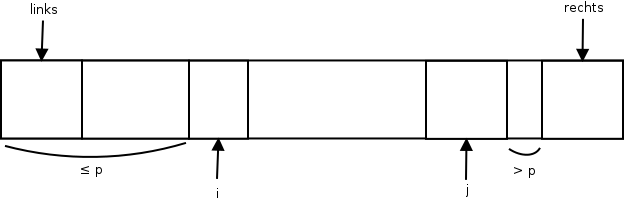
\includegraphics[width=\linewidth]{06/Grafik/img1.png}
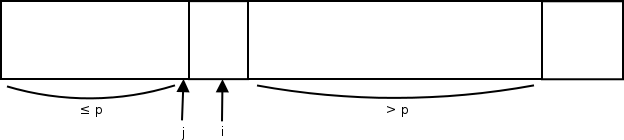
\includegraphics[width=\linewidth]{06/Grafik/img2.png}
\caption{}
\end{wrapfigure}

\vspace{0pt}
\textbf{Schleifen-Invariante:}\\
$a[k] > p~~\text{für}~~j <k<rechts$\\
$a[k] \leq p ~~\text{für}~~links<k<i$ 
\vspace{50pt}

\pagebreak 

\subsection{Zufallspermutation}
\lstinputlisting[language=C, style = pseudo]{06/Code/zufallspermutation.c}

\begin{mdframed}
\subsection{Einschub: Stochastik}
\subsubsection{Fairer Würfel (Erwartungswert):} X sei Zufallsvariable $~\hat{=}~$ Anzahl Augen\\
\[Pr(X=x_i)~~~~x_i \in \{1,2,3,4,5,6\} \]
\[E(X) = \sum_{i=1}^6 x_i \cdot Pr(X=x_i) = \frac{1}{6} \cdot \sum_{i=1}^6 x_i = \frac{1}{6} \cdot \frac{7 \cdot 6}{2} = 3,5 \]

\subsubsection{Fairer Würfel (Erste Sechs):} X sei Zufallsvariable  $~\hat{=}~$ Zahl der benötigten Würfe bis zum Auftreten der ersten 6.
\[x_i \in N\]
\[E(X) = \sum_{i=1}^{\infty} i \cdot Pr(X=i) = \frac{1}{6} \cdot \sum_{i=1}^{\infty} i \cdot \left(\frac{5}{6} \right)^{i-1} \]
Mit der Ableitung der geometrischen Reihe, $\frac{1}{(1-x)^2}$ folgt:\\
\[= \frac{1}{6} \cdot \left(\frac{1}{ \left(1-\frac{5}{6} \right)^2} \right) = 6 \]
\end{mdframed}


\subsection{Laufzeitanalyse}
$T(n) =$ Erwartungswert der Laufzeit von Quicksort bei zufällig gleichverteilter Eingabe-Partition.
\[T(n) = n + \sum_{i=1}^n (T(i-1) + T(n-i)) \cdot \frac{1}{n} \]
\vspace{20pt}
\begin{wrapfigure}[4]{l}{0.6\linewidth}
\vspace{-60pt}
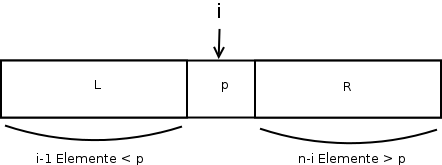
\includegraphics[width=\linewidth]{06/Grafik/img3.png}
\caption{}
\vspace{300pt}
\end{wrapfigure}
Unter der Annahme, dass keine gleich großen Elemente existieren.\\
\\
$T(1) = 0 $
\pagebreak

\paragraph{Lösen durch Einsetzten}
\[T(n) = n + \frac{2}{n} \sum_{i=1}^n T(i-1) = n + \frac{2}{n} \sum_{i=0}^{n-1} T(i)\]
\[ \Leftrightarrow n \cdot T(n) = n^2 + 2 \sum_{i=0}^{n-1} T(i) \]
\[ \Leftrightarrow 2(n-1) \cdot T(n-1) = (n-1)^2 + 2 \sum_{i=0}^{n-2} T(i) \]
\[ \Leftrightarrow (1)-(2) n T(1)-(n-1) T(n-1) = n2 -(n-1)^2 + 2 T(n-1) \]
\[ \Leftrightarrow n T(n) = (n+1) T(n-1) + 2n-1 \]
\[ \Leftrightarrow T(n) \leq \frac{n+1}{n} T(n-1) + 2 \leq \frac{n+1}{2} \left(\frac{n}{n+1} \cdot T(n-2) + 2 \right) + 2 \]
\[ = \frac{n+1}{n-1} T(n-2) + \frac{n+1}{n} \cdot 2 + 2\]
\[ \leq \frac{n+1}{n-1} \left(\frac{n-1}{n-2} T(n-3) +2 \right) + \frac{n+1}{n} \cdot 2 + 2 \cdot 1\]
\[= \frac{n+1}{n-2} T(n-3) + 2 \cdot \frac{n+1}{n-1} + 2 \cdot \frac{n+1}{n} + 2 \cdot \frac{n+1}{n+1} \]
\[ \Rightarrow T(n) \leq \frac{n+1}{n-(k-1)} T(n-k) + 2(n+1) \sum_{i=1}^{k-2} \frac{1}{n-i} ~~~\text{endet für k = n-1}\]
\[ T(n) = 2(n+1) \sum_{i=-1}^{n-3} \frac{1}{n-i} = 2(n+1) \sum_{j=3}^{n+1} \frac{1}{j} \leq 2 (n+1) H_{n+1} \in O(n \log n) ~~~\text{mit j=n-i} \] 

\begin{mdframed}
\paragraph{Einschub: Harmonische Reihe}
\[ H_n = \sum_{i=1}^{n} \frac{1}{i} \]

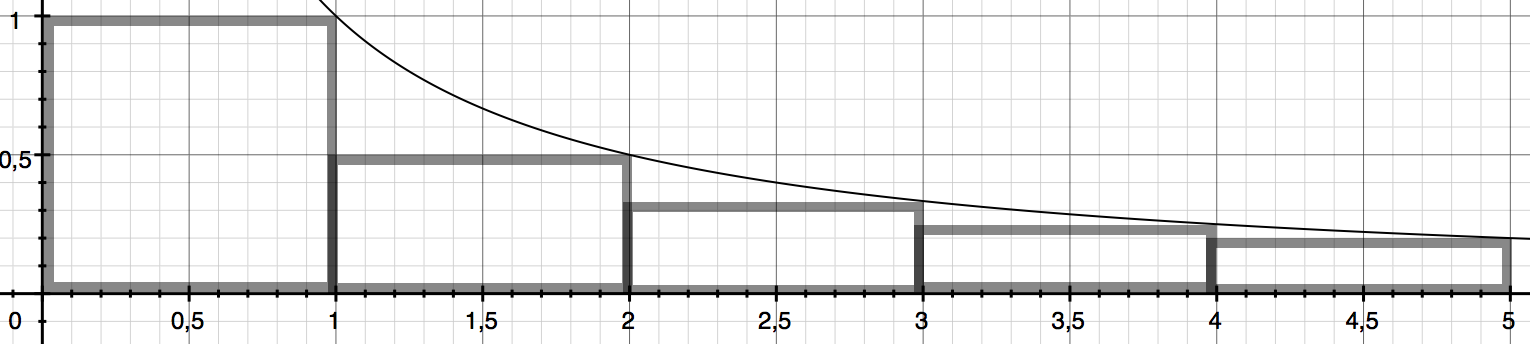
\includegraphics[width=\linewidth]{06/Grafik/img4.png}


\[H_n \leq \int \frac{1}{x} dx +1 = 1 + [\ln x]_1^n = \ln(n)+1 \]
\[\ln(n+1) \leq H_n \leq \ln(n)+1 \]
\end{mdframed}

\pagebreak 

\section{Median in Linearzeit}
Median  $~\hat{=}~ \frac{n}{2} $-kleinste Element in einer Folge von n Elementen

\subsection*{Verallgemeinerung}
Finde das k-t kleinste Elemente in der Folge\\

Naive Strategie: $O(k \cdot n)$


\subsection*{Idee} 

\begin{lstlisting}
select(int[] a, int k) {}
\end{lstlisting}

\begin{wrapfigure}[1]{l}{0.6\linewidth}
\vspace{-25pt}
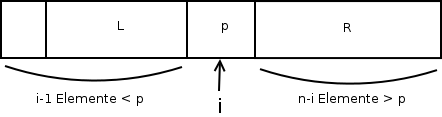
\includegraphics[width=\linewidth]{06/Grafik/img5.png}
\caption{}
\end{wrapfigure}

\vspace{30pt}
Aufruf von Partition
\vspace{90pt}

\paragraph{1. Fall} $k=i \Rightarrow$ Pivotelement war gesucht
\paragraph{2. Fall} $k<i \Rightarrow$ suche rekursiv das k-t kleinste Element in L 
\paragraph{3. Fall} $k>i \Rightarrow$ suche rekursiv das (k-i)-t kleinste Element in R
